Il \textit{GRIDS System} (\textit{Generic Resilient Identity Services}) è un framework che sfrutta il paradigma Social Internet of Things (SIoT) per migliorare le operazioni di mapping ID-to-locator\cite{7983351}, in cui viene disaccoppiato l'host identifier (ID), assegnato univocamente a un oggetto, dal suo locator, cioè l'indirizzo fisico usato a livello di rete per il routing. Di conseguenza, è necessaria una funzione di mapping per tradurre l'ID del nodo di destinazione nel suo locator corrente (per esempio, il suo indirizzo IP): per fare ciò serve un'infrastruttura di mapping distribuita che si basa, per esempio, sulle \textit{Distributed Hash Tables} (DHT) e implica un costo e soprattutto un ritardo addizionale. La richiesta potrebbe attraversare più server prima che arrivi a quello che possiede l'informazione richiesta. L'idea proposta nel GRIDS System è quella di togliere il carico dall'infrastruttura di mapping navigando il grafo SIoT creato dalle relazioni che si stabiliscono tra gli oggetti.

\section{Architettura}
\label{c:grids:arch}

Nella figura \ref{f:grids:arch} è rappresentato uno schema dell'architettura del GRIDS System, in cui ogni nodo GRIDS fornisce un \textit{Relationship Service} (RS), in cui gli elementi sono spiegati più avanti.

\begin{figure}[h!t]
\centerline{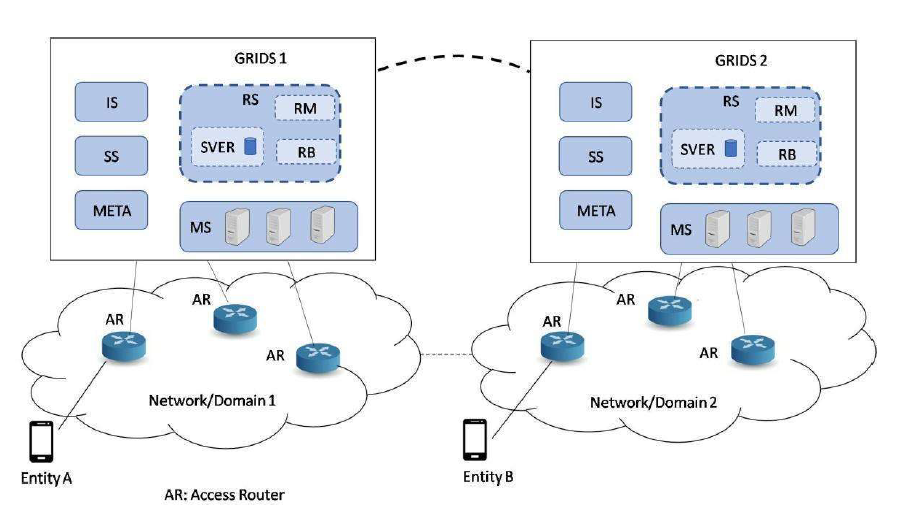
\includegraphics[scale=0.5]{img/GRIDSarch}}
\caption{Architettura del GRIDS System}
\label{f:grids:arch}
\end{figure}

In ogni RS si trova un RM (\textit{Relationship Manager}), un RB (\textit{Relationship Browser}) e uno SVER (\textit{Social Virtual Entity Repository}), i quali sono in run nello stesso server e condividono lo stesso locator nella rete.
I tipi di relazioni che vengono considerate nel sistema sono i seguenti:
\begin{itemize}
    \item \textit{Ownership Object Relationship} (\textbf{OOR}), creata tra oggetti che appartengono allo stesso proprietario;
    \item \textit{Co-location Object Relationship} (\textbf{CLOR}), creata tra dispositivi immobili che si trovano nello stesso luogo. Viene chiamata anche co-geolocation (CGLOR);
    \item Parental Object Relationship (\textbf{POR}), creata tra oggetti con stesso modello, produttore e lotto di produzione;
    \item \textit{Co-work Object Relationship} (\textbf{CWOR}), creata tra oggetti che si "incontrano" tra loro nel posto di lavoro del proprietario, come ad esempio il PC portatile e la stampante in un ufficio;
    \item \textit{Social Object Relationship} (\textbf{SOR}), creata come conseguenza di incontri frequenti tra oggetti, come succede tra smartphone che appartengono a persone che utilizzano lo stesso mezzo di trasporto pubblico ogni giorno per andare a lavoro/scuola, o persone che frequentano lo stesso bar/palestra/ristorante;
    \item \textit{Untrusted Object Relationship} (\textbf{UOR}), si riferisce a relazioni per dispositivi appena aggiunti per avere accesso alla rete sociale, come succede per esempio durante la connessione a uno stesso AP, oppure con i dispositivi nello stesso SVER;
    \item \textit{Transactional Object Relationship} (\textbf{TOR}), si origina quando due o più risorse interagiscono tra loro, come due persone che hanno una chiamata VoIP, una persona che ha accesso alle informazioni fornite da un sensore, due web service che si scambiano servizi, ecc.
\end{itemize}

\subsection{Relationship Manager}
\label{c:grids:rm}

La relazione tra due entità (e quindi tra le rispettive SVE) viene stabilita in modalità diverse, a seconda del tipo di relazione in questione. Alcune di esse (per esempio la OOR oppure la POR) sono legate al profilo della SVE, mentre altre dipendono dal comportamento dei dispositivi stessi (per esempio la SOR o la CLOR). Tutte queste informazioni vengono trasmesse tramite tag e metadata al RM, il quale deve processarle per stabilire le azioni di management da fare. 

\begin{figure}[h!t]
\centering
\subfloat[Elementi del RM]{
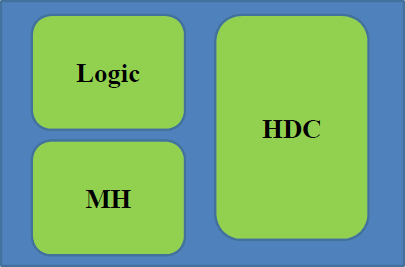
\includegraphics[height=100pt]{img/rma}
\label{f:grids:rma}}
\qquad
\subfloat[Componenti della logica del RM]{
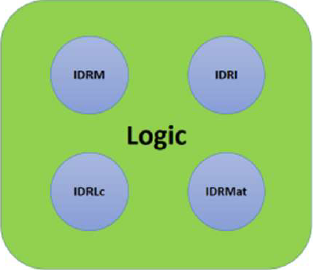
\includegraphics[height=100pt]{img/rmb}
\label{f:grids:rmb}}
\caption{Relationship Manager}
\label{f:grids:rm}
\end{figure}

Il RM è costituito da tre parti, come raffigurato nella figura \ref{f:grids:rma}. Gli algoritmi decisionali e i classificatori sono implementati nel modulo Logic, attraverso l'analisi dei tags e dei metadata delle SVE. Le informazioni utili per identificare le relazioni sono conservate temporaneamente nella \textit{Historical Data Cache} (HDC). Il \textit{Message Handler} (MH), infine, inoltra l'informazione sulle nuove relazioni ad altri RM affinch\'e le friendiship table delle SVE siano aggiornate, nel caso in cui le due SVE sono gestite da due diversi RM. Il MH, inoltre, pubblica i metadata e i tag dei \textit{monitored events}, i quali possono innescare la creazione/cancellazione di una nuova relazione e iscriversi all'evento stesso.

Gli elementi principali che compongono la logica del RM sono i seguenti (figura \ref{f:grids:rmb}):

\begin{itemize}
    \item \textit{ID Relation Initialization} (IDRI): inizializza le \textit{Friend Table} (FT) durante la registrazione di nuove entità, aggiungendo le prime relazioni (come OOR/POR/UOR) con le altre entità all'interno dello stesso SVER;
    \item \textit{ID Relation Management} (IDRM): implementa gli algoritmi e le procedure per stabilire, aggiornare ed eliminare le relazioni;
    \item \textit{ID Relation Lifecycle} (IDLc): valuta il lifecycle delle entittà gestite e fornisce statistiche rigurado le attività e i risultati dell'IDRM;
    \item \textit{ID Relation Maturity} (IDRMat): questo elemento interagisce con l'elemento incaricato di valutare l'affidabilità delle altre entità, per aggiornare di conseguenza i pesi delle relazioni.
\end{itemize}

\begin{figure}[h!t]
\centerline{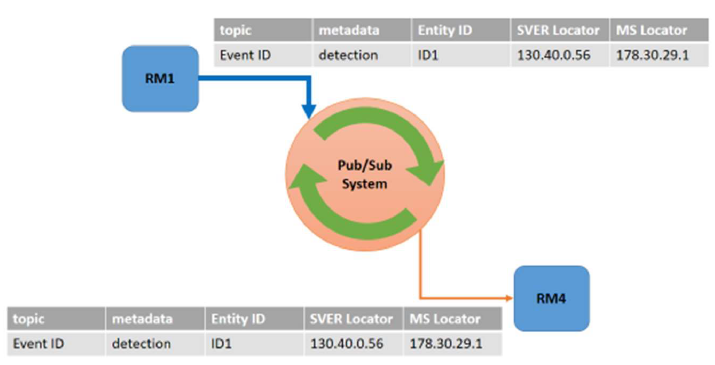
\includegraphics[scale=0.5]{img/scambiomessaggi}}
\caption{Propagazione degli eventi}
\label{f:grids:scambiomex}
\end{figure}

Le funzioni di \textit{relationship management} si affidano su due procedure di message forwarding, che sono le seguenti:

\begin{itemize}
    \item \textit{New friendship alert}: generato e ricevuto quando viene stabilita un'amicizia tra due SVE che risiedono in diversi RM. Di conseguenza, un RM invia all'altro informazioni come: Entity ID, metadati, tipo di relazione, SVE locator e il locator del GRIDS-MS locator dell'amico che deve essere aggiunto nella FT della SVE di destinazione;
    \item \textit{Event alert}: trasmette informazioni circa alcuni eventi relativi a una SVE e che potrebbe causare la creazione di una nuova relazione. Queste informazioni devono essere valutate dai RM delle entità coinvolte (o dal singolo RM se le SVE risiedono nello stesso RM). Visto che non sempre sono noti i RM interessati a certi eventi, questa informazione dovrebbe essere diffusa a tutti i RM potenzialmente interessati. per fare ciò si utilizza il Pub/Sub System (PSS), come mostrato nella figura \ref{f:grids:scambiomex}. L'EventID in figura identifica l'argomento di interesse, per esempio: EventID=“AP address A677.7BCD.F345”. Questa informazione viene diffusa cosicch\'e gli altri RM sanno che quell'entità ricade sotto la copertura dell'AP con MAC address A677.7BCD.F345.
\end{itemize}

\section{Implementazione}
\label{c:grids:implementation}

L'implementazione del GRIDS System è stata realizzata nel linguaggio Java. Nello specifico, è stato utilizzato Java Enterprise Edition per creare una Web Application, la quale è stata deployata su un Application Server: nel nostro caso si tratta di Glassfish 5.0.0, che è pensato appositamente per le implementazioni della Java Platform.

Il sistema è distribuito su più macchine, le quali comunicano tramite RMI\footnote{https://docs.oracle.com/javase/tutorial/rmi/index.html} (\textit{Remote Method Invocation}), una tecnologia il cui scopo è quello di rendere trasparenti al programmatore i dettagli della comunicazione in rete. I nodi prendono il nome di Server, e sono interconnessi tra loro per formare una rete peer-to-peer. Ognuno di essi viene identificato dal Server ID.

La classe in cui vengono definiti i metodi remoti è \textit{GridsSystem}, che implementa l'interfaccia root RMI. Nel listing \ref{gridssys} è riportata la struttura del codice di questa classe.

La classe \textit{CustomSimulation} contiene il metodo initNetwork() per inizializzare il Server: viene creata un'istanza di GridsSystems e viene effettuato il lookup dell'interfaccia RMI remota per la registrazione del server, richiamando il metodo remoto della classe GridsSystem. Il tutto viene avviato tramite la GUI contenuta nella classe \textit{EngineSimulator}, mostrata nel paragrafo successivo in figura \ref{f:grids:gui1}.
Sempre nella funzione initNetwork() vengono instaurate le relazioni tra i nodi, in pieno accordo con il paradigma Social IoT. I parametri utilizzati nella creazione delle relazioni sono le coordinate geografiche dei nodi (che si ottengono dalle informazioni contenute nelle piattaforme IoT che "ospitano" i nodi) e le probabilità di creazione delle relazioni (fornite attraverso il file di configurazione \textit{probabilities.ini}). Per esigenze di testing, i tipi di relazioni (come ad esempio OOR, SOR, CLOR) sono assegnati casualmente.

\begin{lstlisting}[caption={GridsSystem.java},label={gridssys},style={c}]

public class GridsSystems extends UnicastRemoteObject implements RMIRootInterface {

    HashMap<String, String> servers_address;

    public GridsSystems() throws RemoteException {
        super();
        servers_address = new HashMap<>();
    }

    @Override
    public void RegisterServer_address(String address, String id) {
        this.servers_address.put(address, id);
        System.out.println("SERVER REGISTERED: " + "//" + address + "/server" + id + "\n");
    }
\end{lstlisting}

Oltre queste, è disponibile una risorsa REST per poter consultare i dati non solo del Server corrente, ma anche degli altri Server attivi nel sistema. Le chiamare HTTP disponibili sono le seguenti:

\begin{itemize}
    \item GET all'indirizzo "/Sim/SIoT/Server/{id}/SVER/{uid}" per ricevere la lista delle relazioni del nodo \textit{uid} contenuto nello SVER del server \textit{id};
    \item GET a "/Sim/SIoT/Server/{id}/{uid}" per ottenere le proprietà della singola SVE (id e uid come la richiesta sopracitata);
    \item GET a "/Sim/SIoT/Server/{id}/Clients" per ottenere l'elenco dei Client contenuti nel server {id};
    \item GET al path "/Sim/SIoT/Server/0/Entities" per BOH. 
    
\end{itemize}

Ciò è possibile grazie alla presenza del database MySQL con cui il sistema interagisce attraverso la classe \textit{GridsRS}, ossia il Relationship Manager della specifica, e alla classe \textit{Server}. Quest'ultima implementa un'ulteriore interfaccia RMI, riportata qui di seguito nel listing \ref{rmiInterface}.

\begin{lstlisting}[caption={RMIInterface.java},label={rmiInterface},style={c}]

public interface RMIInterface extends Remote {

    public RelBrowser getRelBrowser() throws RemoteException;
    public HashSet<HashMap> getGRIDS_MS() throws RemoteException;
    public void addMap_GRIDS(HashMap map) throws RemoteException;
    public HashMap<ClientInterface, Sve> getGRIDS_RS() throws RemoteException;
    public void updateGRIDS_RS(ClientInterface c, Sve sve) throws RemoteException;
    public void fillGRIDS_RS() throws RemoteException;
}
\end{lstlisting}

La classe \textit{Server} contiene anche gli attributi che caratterizzano il nodo stesso, i quali sono: l'ID, l'indirizzo IP, il GridsRS, il GridsMS (\textit{GRIDS Mapping Service}), che di fatto realizza la corrispondenza tra ID del nodo e indirizzo IP corrispondente, e il \textit{RelBrowser}, che è l'oggetto responsabile della navigazione nel grafo delle relazioni sociali tra i nodi.
Oltre al \textit{RelBrowser}, altre classi utili per la navigazione delle relazioni sociali sono \textit{FriendTableEntry} e \textit{SVE}, che saranno descritte più avanti.

Per poter accedere ai dati predenti nei canali Thingspeak o alle risorse di FESTIVAL sono disponibili delle librerie apposite.

Per quanto riguarda il livello di \textit{Data Access}, essa è composta da due database: \textit{social\_iot\_platform} e \textit{social\_iot\_platform\_sve}. Il primo contiene la tabella denominata sver, la quale contiene l'elenco dei Client che fanno riferimento allo stesso SVER, che di fatto è il Server che contiene la tabella stessa. Le colonne sono composte dai seguenti campi:

\begin{itemize}
    \item \textbf{channel}: codice che identifica, nel caso in cui il nodo sia virtualizzato da Thingspeak, il canale della piattaforma:
    \item \textbf{uid}: ID del client;
    \item \textbf{areas}: coordinate geografiche nelle quali è posizionato il nodo;
    \item \textbf{ip}: sempre nel caso si tratti di Thingspeak, è l'indirizzo web del nodo (ad esempio: https://thingspeak.com/channels/156761);
    \item \textbf{meta}: eventuali metadati (ad esempio una descrizione del nodo);
    \item \textbf{server}: ID del server che contiene la SVE;
\end{itemize}

Il database \textit{social\_iot\_platform\_sve}, invece, contiene un numero di tabelle pari al numero di Client nello SVER, all'interno delle quali si trova l'elenco degli amici della SVE. Le colonne di ogni tabella sono:

\begin{itemize}
    \item \textbf{ifFriend}: uid della SVE con cui è definita la relazione;
    \item \textbf{REL}: tipo di relazione costituita;
    \item \textbf{MS\_LOCATOR}: indirizzo IP del Server che fa da GridsMS per il nodo "amico"; 
    \item \textbf{SVE\_LOCATOR}: indirizzo IP in cui si trova la SVE 
    \item \textbf{Server}: ID del Server in cui si trova la SVE dell'"amico".
\end{itemize}

Le classi necessarie per realizzare il mapping con il database sono le seguenti: 
\begin{itemize}
    \item la classe \textit{Client}, che mappa le SVE, in particolare i record della tabella sver;
    \item la classe \textit{FriendTableEntry}, che rappresenta il singolo record contenuto nelle tabelle del database social\_iot\_platform\_sve;
    \item \textit{SVE}, lista di FriendTableEntry.
\end{itemize}

Notare che, anche se contengono dati diversi, le classi Client e SVE rappresentano lo stesso concetto: la virtualizzazione del nodo IoT visto sia come entità sociale, sia come semplice dispositivo.

Il driver utilizzato per l'interazione tra il codice Java e il database MySQL è JDBC\footnote{https://www.oracle.com/technetwork/java/javase/jdbc/index.html} (\textit{Java Database Connectivity}), che fornisce una serie di API per effettuare query e per aggiornare dati in un database, ed è orientato per database relazionali.

In figura \ref{f:grids:diagramma} è possibile osservare il diagramma delle classi principali dell'architettura del Grids System. Notare che sono raffigurate soltanto le classi, i metodi e gli attributi necessari per la descrizione del sistema: le classi delle librerie di Thingspeak e FESTIVAL, per esempio, sono state omesse per semplicità.


\begin{figure}[h!t]
\centerline{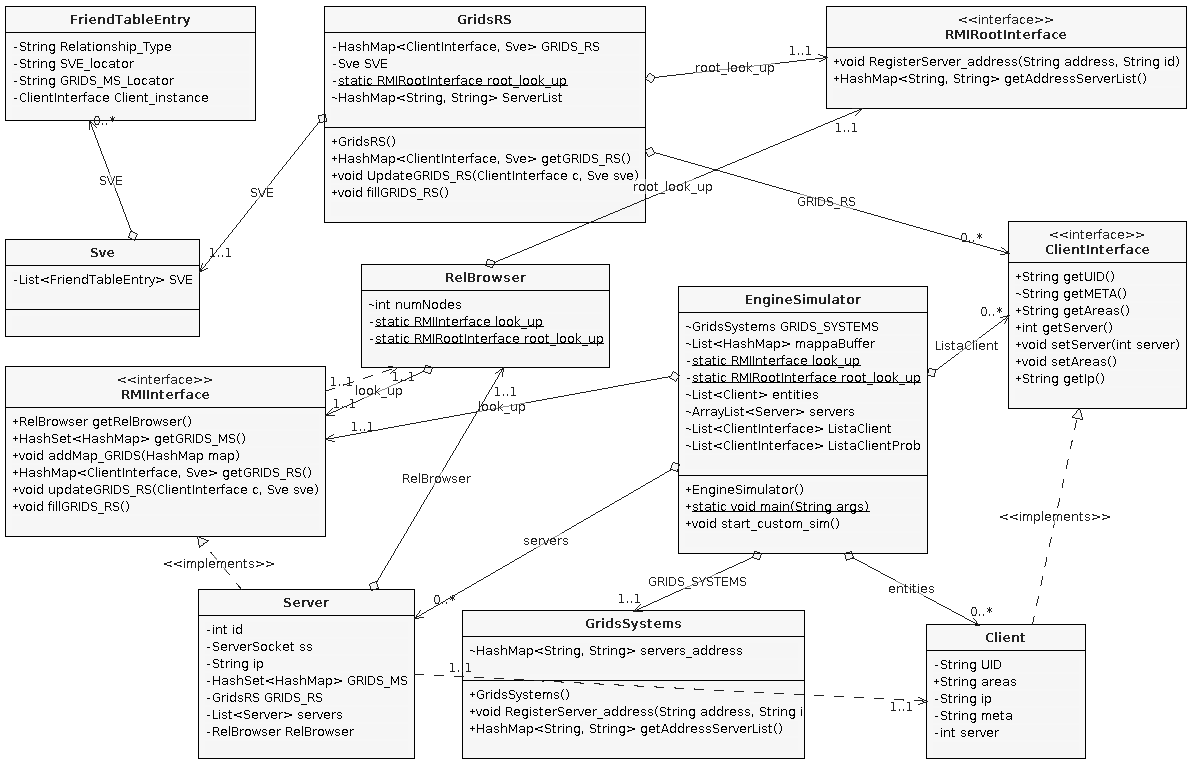
\includegraphics[width=\textwidth]{img/initialDiagramCorrect}}
\caption{Diagramma delle classi del Grids System}
\label{f:grids:diagramma}
\end{figure}


\section{Caso d'uso d'esempio}
\label{c:grids:usecase}

Per effettuare il deployment della piattaforma è necessario aprire il progetto Java con un IDE, in questo caso Netbeans IDE 8.2. Bisogna inoltre assicurarsi che il database sia in run: è possibile utilizzare XAMPP per Linux 5.6.20, che permette di avviare velocemente non solo MySQL, ma anche server Apache e i linguaggi di programmazione PHP e Perl, utili per lo sviluppo di semplici applicazioni Web (nonostante ciò, questi ultimi non sono necessari per l'avvio del Grids System). 

Fatto ciò, bisogna settare correttamente gli indirizzi IP di Server, Gateway e SVER e l'ID del server. Nel caso d'uso base, visto che il Server avviato è solo uno, l'ID è pari a 0. 

\begin{figure}[h!t]
\centerline{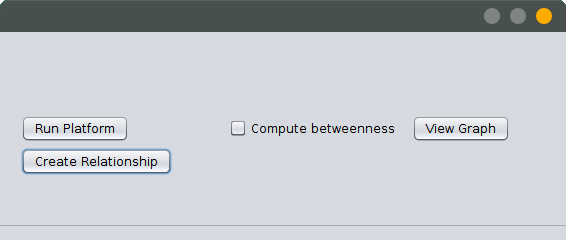
\includegraphics[scale=2.5]{img/gui1}}
\caption{GUI del Grids System}
\label{f:grids:gui1}
\end{figure}

Poi bisogna avviare il progetto, il quale verrà deployato sul Glassfish server, e l'interfaccia grafica, raffigurata in figura \ref{f:grids:gui1}.
Per avviare la piattaforma, bisogna cliccare sugli appositi jButton \textit{Run Platform} e \textit{Create Relationship}, rispettivamente per effettuare la configurazione RMI e per creare le relazioni tra le Social Virtual Entities. Infine, cliccando sul tasto \textit{View Graph} è possibile visualizzare il grafo delle relazioni, come raffigurato in figura \ref{f:grids:gui2}. È possibile selezionare i singoli nodi del grafo per visualizzare un'ulteriore finestra in cui sono contenute le informazioni della SVE corrispondente.

\begin{figure}[h!t]
\centerline{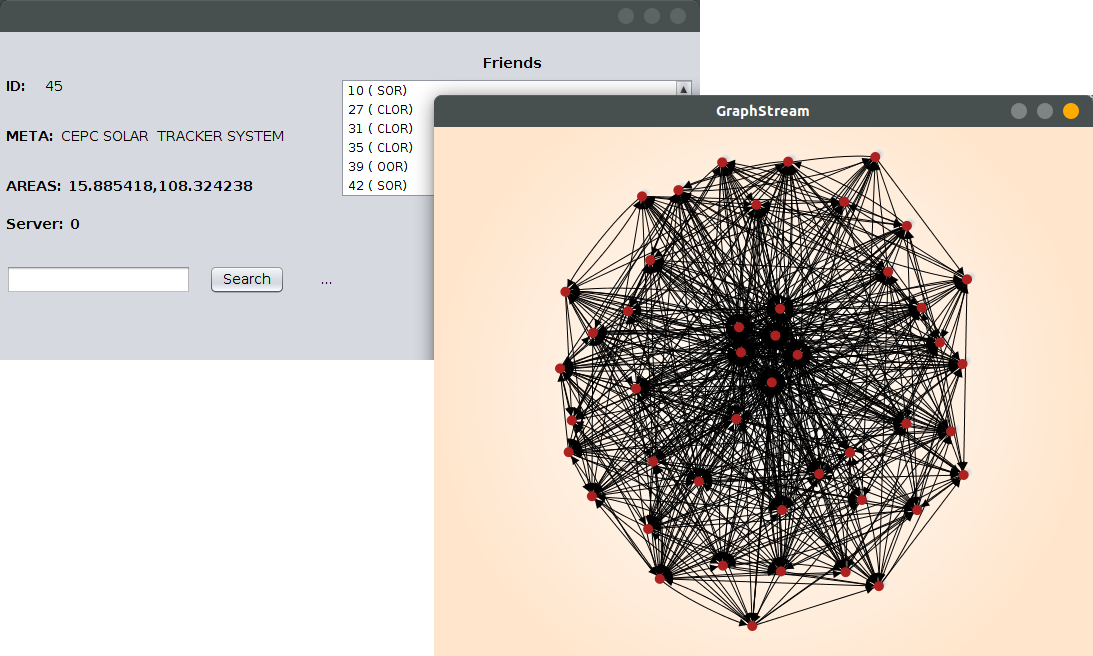
\includegraphics[width=\textwidth]{img/gui2}}
\caption{Grafo delle relazioni SIoT}
\label{f:grids:gui2}
\end{figure}

Nel capitolo successivo, la struttura appena presentata verrà ampliata e arricchita per contenere un wallet Bitcoin, e quindi la possibilità di ricevere denaro dagli utenti che si connetteranno alla rete SIoT e di inviarlo ai proprietari di \textit{smart devices} che espongono tramite questa piattaforma.